\documentclass[10pt]{exam}

\usepackage{amssymb, amsmath, amsthm, mathrsfs, multicol, graphicx}
\usepackage{tikz}
\usepackage{pgf}

 \def\d{\displaystyle}
\def\?{\reflectbox{?}}
\def\b#1{\mathbf{#1}}
\def\f#1{\mathfrak #1}
\def\c#1{\mathcal #1}
\def\s#1{\mathscr #1}
\def\r#1{\mathrm{#1}}
\def\N{\mathbb N}
\def\Z{\mathbb Z}
\def\Q{\mathbb Q}
\def\R{\mathbb R}
\def\C{\mathbb C}
\def\F{\mathbb F}
\def\A{\mathbb A}
\def\X{\mathbb X}
\def\E{\mathbb E}
\def\O{\mathbb O}
\def\U{\mathcal U}
\def\pow{\mathcal P}
\def\inv{^{-1}}
\def\nrml{\triangleleft}
\def\st{:}
\def\~{\widetilde}
\def\rem{\mathcal R}
\def\sigalg{$\sigma$-algebra }
\def\Gal{\mbox{Gal}}
\def\iff{\leftrightarrow}
\def\Iff{\Leftrightarrow}
\def\land{\wedge}
\def\And{\bigwedge}
\def\AAnd{\d\bigwedge\mkern-18mu\bigwedge}
\def\Vee{\bigvee}
\def\VVee{\d\Vee\mkern-18mu\Vee}
\def\imp{\rightarrow}
\def\Imp{\Rightarrow}
\def\Fi{\Leftarrow}

%\def\={\equiv}
\def\var{\mbox{var}}
\def\mod{\mbox{Mod}}
\def\Th{\mbox{Th}}
\def\sat{\mbox{Sat}}
\def\con{\mbox{Con}}
\def\bmodels{=\joinrel\mathrel|}
\def\iffmodels{\bmodels\models}
\def\dbland{\bigwedge \!\!\bigwedge}
\def\dom{\mbox{dom}}
\def\rng{\mbox{range}}
\DeclareMathOperator{\wgt}{wgt}


\def\bar{\overline}


\newcommand{\vtx}[2]{node[fill,circle,inner sep=0pt, minimum size=4pt,label=#1:#2]{}}
\newcommand{\va}[1]{\vtx{above}{#1}}
\newcommand{\vb}[1]{\vtx{below}{#1}}
\newcommand{\vr}[1]{\vtx{right}{#1}}
\newcommand{\vl}[1]{\vtx{left}{#1}}
\renewcommand{\v}{\vtx{above}{}}

\def\circleA{(-.5,0) circle (1)}
\def\circleAlabel{(-1.5,.6) node[above]{$A$}}
\def\circleB{(.5,0) circle (1)}
\def\circleBlabel{(1.5,.6) node[above]{$B$}}
\def\circleC{(0,-1) circle (1)}
\def\circleClabel{(.5,-2) node[right]{$C$}}
\def\twosetbox{(-2,-1.4) rectangle (2,1.4)}
\def\threesetbox{(-2.5,-2.4) rectangle (2.5,1.4)}
\newcommand{\twoline}[2]{\begin{pmatrix}#1 \\ #2 \end{pmatrix}}


\def\circleA{(-.5,0) circle (1)}
\def\circleAlabel{(-1.5,.6) node[above]{$A$}}
\def\circleB{(.5,0) circle (1)}
\def\circleBlabel{(1.5,.6) node[above]{$B$}}
\def\circleC{(0,-1) circle (1)}
\def\circleClabel{(.5,-2) node[right]{$C$}}
\def\twosetbox{(-2,-1.5) rectangle (2,1.5)}
\def\threesetbox{(-2,-2.5) rectangle (2,1.5)}

%\pointname{pts}
\pointsinmargin
\marginpointname{pts}
\addpoints
\pagestyle{head}
\printanswers

\firstpageheader{Math 228}{\textbf{Homework 1 Solutions}}{Due: Wednesday, August 29}


\begin{document}
% \noindent \textbf{Instructions}: Complete the homework problems below on {\em separate} sheets of paper (and not all jammed up between the questions).  This is to be turned in and graded, so make sure your work is neat and easy to read -- there is nothing wrong with using a \underline{separate sheet} of paper for each problem. Your work will be graded on correctness as well as the clarity of your explanations.  You may work with other students in this class on solving the problems, but your write-ups should be completed individually.  You are not permitted to search for solutions online or in other textbooks.

\begin{questions}

	\question[6] A graph is a way of representing the relationships between elements in a set: an edge between the vertices $x$ and $y$ tells us that $x$ is related to $y$ (which we can write as $x \sim y$).  Not all sorts of relationships can be represented by a graph though.  For each relationship described below, either draw the graph or explain why the relationship cannot be represented by a graph.
	\begin{parts}
		\part The set $V = \{1,2, \ldots, 9\}$ and the relationship $x \sim y$ when $x-y$ is a non-zero multiple of 3.
		\begin{solution}
			This will be a graph.  The graph will consist of three triangles. %Draw graph.
			\begin{center}
				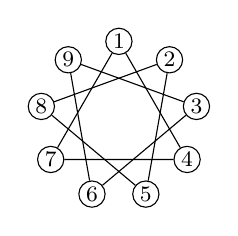
\begin{tikzpicture}
					\foreach \x in {1,...,9}{
					\node[fill=white,draw,circle,inner sep=1pt] at (130-\x*40:1) (a\x) {\footnotesize $\x$};
					}
					\draw (a1) -- (a4) -- (a7) -- (a1);
					\draw (a2) -- (a5) -- (a8) -- (a2);
					\draw (a3) -- (a6) -- (a9) -- (a3);
				\end{tikzpicture}
			\end{center}
		\end{solution}
		\part The set $V = \{1,2, \ldots, 9\}$ and the relationship $x \sim y$ when $y$ is a multiple of $x$.
		\begin{solution}
			This relationship does not give a graph.  For example, $2 \sim 4$ but $4 \not\sim 2$.  However, this would give a directed graph.
		\end{solution}
		\part The set $V = \{1,2,\ldots, 9\}$ and the relationship $x \sim y$ when $0 < |x-y| < 3$.
		\begin{solution}
			This will give a graph.  Each vertex will be adjacent to the vertices 1 or 2 spaces to the left or right.  %Draw graph.
			\begin{center}
				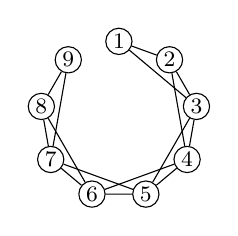
\begin{tikzpicture}
					\foreach \x in {1,...,9}{
					\node[fill=white,draw,circle,inner sep=1pt] at (130-\x*40:1) (a\x) {\footnotesize $\x$};
					}
					\draw (a1) -- (a2) -- (a3) -- (a4) -- (a5) -- (a6) -- (a7) -- (a8) -- (a9);
					\draw (a1) -- (a3) -- (a5) -- (a7) -- (a9);
					\draw (a2) -- (a4) -- (a6) -- (a8);
				\end{tikzpicture}
			\end{center}
		\end{solution}
	\end{parts}





	\question[6] Consider the graphs $G_1 = (V_1,E_1)$ and $G_2 = (V_2, E_2)$:\\
	$G_1$: $V_1=\{a,b,c,d,e,f,g\}$, $E_1=\{\{a,b\},\{a,d\},\{b,c\},\{b,d\},\{b,e\},\{b,f\},\{c,g\},\{d,e\},\{e,f\},\{f,g\}\}$.\\
	$G_2$: $V_2=\{v_1,v_2,v_3,v_4,v_5,v_6,v_7\}$,

	\hspace{1.75em} $E_2=\{\{v_1,v_4\},\{v_1,v_5\},\{v_1,v_7\},\{v_2,v_3\},\{v_2,v_6\},\{v_3,v_5\},\{v_3,v_7\},\{v_4,v_5\},\{v_5,v_6\},\{v_5,v_7\}\}$.
	\begin{parts}
	\part Let $f:G_1 \rightarrow G_2$ be a function that takes the vertices of $G_1$ to vertices of $G_2$.  The function is given by the following table:

	\begin{center}
	\begin{tabular}{c*{7}{|c}}
	$x$ & $a$ & $b$ & $c$ & $d$ & $e$ & $f$ & $g$ \\ \hline
	$f(x)$ & $v_4$ & $v_5$ & $v_1$ & $v_6$ & $v_2$ & $v_3$ & $v_7$
	\end{tabular}
	\end{center}
	%
	%\[f(a)=v_4\]
	%\[f(b)=v_5\]
	%\[f(c)=v_1\]
	%\[f(d)=v_6\]
	%\[f(e)=v_2\]
	%\[f(f)=v_3\]
	%\[f(g)=v_7\]
	Is $f$ an isomorphism between $G_1$ and $G_2$? Explain.
	\begin{solution}
	Recall that in order for $f$ to be an isomorphism between $G1$ and $G2$, it must preserve relationships between vertices. To put this into context, this means that since $a$ and $b$ are joined via an edge in $G1$ that their corresponding vertices in $G_2$ must also be joined by an edge. This must be true for all of the vertices and edges. When examining the function, we can see that the vertex $g$ goes to $v_7$, that is $f(g)=v_7$. BUT, $g$ has exactly 2 edges (so $g$ is degree 2) and $v_7$ is degree 3. This means that $f$ cannot possibly be an isomorphism. Similarly, we can see that $f$ does not take $c$ to the correct vertex either $c$ is degree 2 and $v_1$ has degree 3.
	\end{solution}
	\part Define a function $g$ (different from $f$) that \emph{is} an isomorphism between $G_1$ and $G_2$.
	\begin{solution}
	\begin{center}
	\begin{tabular}{c*{7}{|c}}
	$x$ & $a$ & $b$ & $c$ & $d$ & $e$ & $f$ & $g$ \\ \hline
	$g(x)$ & $v_4$ & $v_5$ & $v_6$ & $v_1$ & $v_7$ & $v_3$ & $v_2$
	\end{tabular}
	\end{center}
	\end{solution}
	\part Is the graph pictured below isomorphic to $G_1$ and $G_2$? Explain.
	\begin{center}
	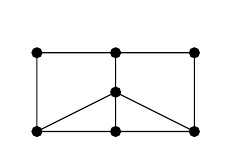
\begin{tikzpicture}
	\draw (-1, 0) coordinate (v1) -- (0,0) coordinate (v2) -- (1,0) coordinate (v3) -- (1,1) coordinate (v4) -- (0,1) coordinate (v5) -- (-1,1) coordinate (v6) -- (v1) --(0,.5) coordinate (v7) -- (v2) (v7) -- (v3) (v7) -- (v5);
	\foreach \i in {1,...,7}{
		\fill (v\i) \v;
	}
	\end{tikzpicture}
	\begin{solution}
	No, it could not possibly be isomorphic. If you count up the degrees of each vertex in this picture, you can see that the highest degree is 4 (the center vertex). In order to be isomorphic to either $G_1$ or $G_2$ we would definitely need a vertex of degree 5, which we don't have.
	\end{solution}

	\end{center}

	\end{parts}


	\question[8] Decide whether the statements below about subgraphs are true or false.  For those that are true, briefly explain why (1 or 2 sentences).  For any that are false, give a counterexample.
	\begin{parts}
		\part Any subgraph of a complete graph is also complete.
		\begin{solution}
			False.  For example, if you remove one edge from $K_4$, you no longer have a complete graph.
		\end{solution}
		\part Any \emph{induced} subgraph of a complete graph is also complete.
		\begin{solution}
			True.  To get an induced subgraph, you can remove some vertices, but you must keep all the edges you can.  Whatever edges you are left with will all be connected by edges, so a complete graph.
		\end{solution}
		\part Any subgraph of a bipartite graph is bipartite.
		\begin{solution}
			True.  A bipartite graph is one in which it is possible to partition the vertices into two sets with no edges between vertices in the same set.  Since you do not add edges when forming a subgraph, you will always have the two sets.
		\end{solution}
		\part Any subgraph of a tree is a tree.
		\begin{solution}
			False.  You could remove vertices or edges that would disconnect the tree.  It is true that the subgraph could not have any cycles, so we could say that any subgraph of a tree is a forest.
		\end{solution}
	\end{parts}


\question[10] We often define graph theory concepts using set theory.  For example, given a graph $G = (V, E)$ and a vertex $v \in V$, we define
\[N(v) = \{u \in V \st \{v,u\} \in E\}.\]
We define $N[v] = N(v) \cup \{v\}$.  The goal of this problem is to figure out what all this means.
\begin{parts}
	\part Let $G$ be the graph with $V = \{a,b,c,d,e,f\}$ and \\$E = \{\{a,b\}, \{a,e\},\{b, c\}, \{b,e\}, \{c,d\}, \{c, f\}, \{d, f\}, \{e,f\}\}$.  Find $N(a)$, $N[a]$, $N(c)$, and $N[c]$.
	\begin{solution}
		$N(a) = \{b, e\}$, $N[a] = \{a,b,e\}$.  $N(c) = \{b, d, f\}$ and $N[c] = \{b,c,d,f\}$.
	\end{solution}
	\part What is the largest and smallest possible values for $|N(v)|$ and $|N[v]|$ for the graph in part (a)?  Explain.
	\begin{solution}
		We have $2 \le |N(v)| \le 3$ and $3 \le |N[v]| \le 4$
	\end{solution}
	\part Give an example of a graph $G = (V, E)$ (probably different than the one above) for which $N[v] = V$ for some vertex $v \in V$.  Is there a graph for which $N[v] = V$ for \emph{all} $v \in V$?  Explain.
	\begin{solution}
		We need one vertex to be adjacent to every other vertex.  For example, a star graph.  However, we can make every vertex adjacent to every other vertex ($K_n$ for each $n$) to make $N[v] = V$ for \emph{all} $v \in V$.
	\end{solution}
	\part Give an example of a graph $G = (V,E)$ for which $N(v) = \emptyset$ for some $v \in V$.  Is there an example of such a graph for which $N[u] = V$ for some other $u \in V$ as well?  Explain.
	\begin{solution}
		Such a vertex $v$ must not be adjacent to anything else (it is an \emph{isolated vertex}).  For example, $V = \{a,b,c\}$ and $E = \{\{a,b\}\}$ has $N(v) = \emptyset$.

		Note that if there is an isolated vertex, then there cannot be a vertex adjacent to every other vertex, so you cannot also have $N[u] = V$.
	\end{solution}
	\part Describe in words what $N(v)$ and $N[v]$ mean in general.
	\begin{solution}
		$N(v)$ is the set of all vertices adjacent to $v$, and $N[v]$ is this set together with $v$.    We usually call $N(v)$ the \emph{open neighborhood of $v$}, and $N[v]$ the \emph{closed neighborhood} of $v$.  You could also say that $N(v)$ is the set of vertices exactly distance one from $v$, and $N[v]$ the set of vertices \emph{at most} distance one away from $v$ (where $v$ is distance 0 from $v$).
	\end{solution}
\end{parts}




\end{questions}




\end{document}
